\subsection{Chaining blocks}
\label{subsect-chain-exp}
In the next synthetic experiments we show that MultiChain can create a chain of blocks between two peers.
The experiments are run using gumby.
In the first synthetic experiment we try to create 10 subsequent blocks simulate a download of 10 MB with a speed of 1000 KB/s.
The scheduler waits for 1 MB uploaded to another peer before scheduling a block.
The result of the experiment can be seen in the graph in Figure \ref{fig:chain-experiment-graph}.
In this graph it can be clearly seen that MultiChain is succesful in creating a chain of 10 blocks.

\begin{figure}[!h]
	\centerline{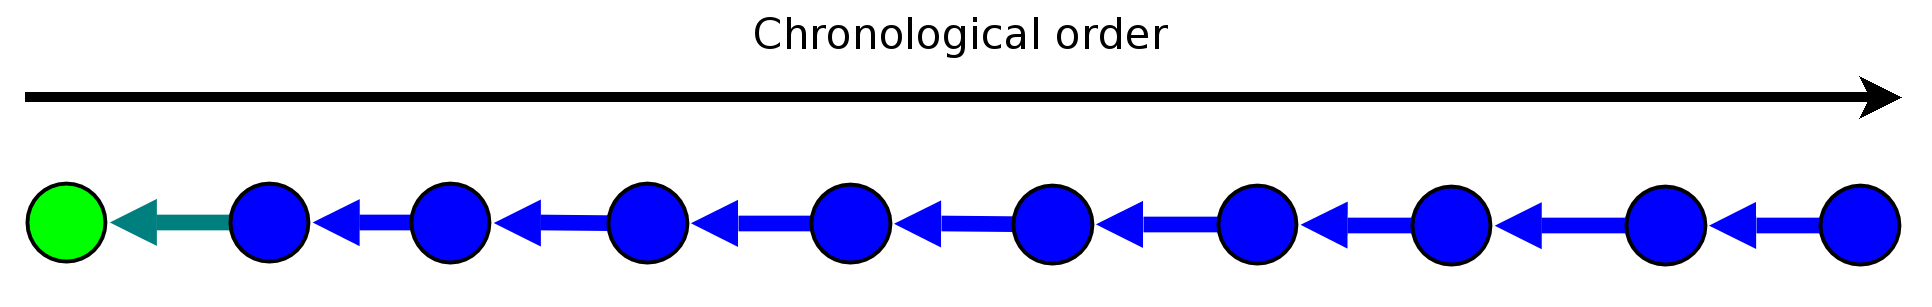
\includegraphics[scale=0.20]{experimentation/chain/chain.png}}
	\caption{MultiChain chain graph of a single download of 10 MB.}
	\label{fig:chain-experiment-graph}
\end{figure}

The download amount stored in each block for the downloader is plotted in Figure \ref{fig:chain-experiment-amounts-small}.
These datapoints are connected by a dotted line representing the link between these blocks.
These plots show that MultiChain correctly tracks the download of 10 MB.
The slope of the figure corresponds with the speed of the download.
The upload amount of every seeder is identical to the amount of download of the downloader.

\begin{figure}
\centerline{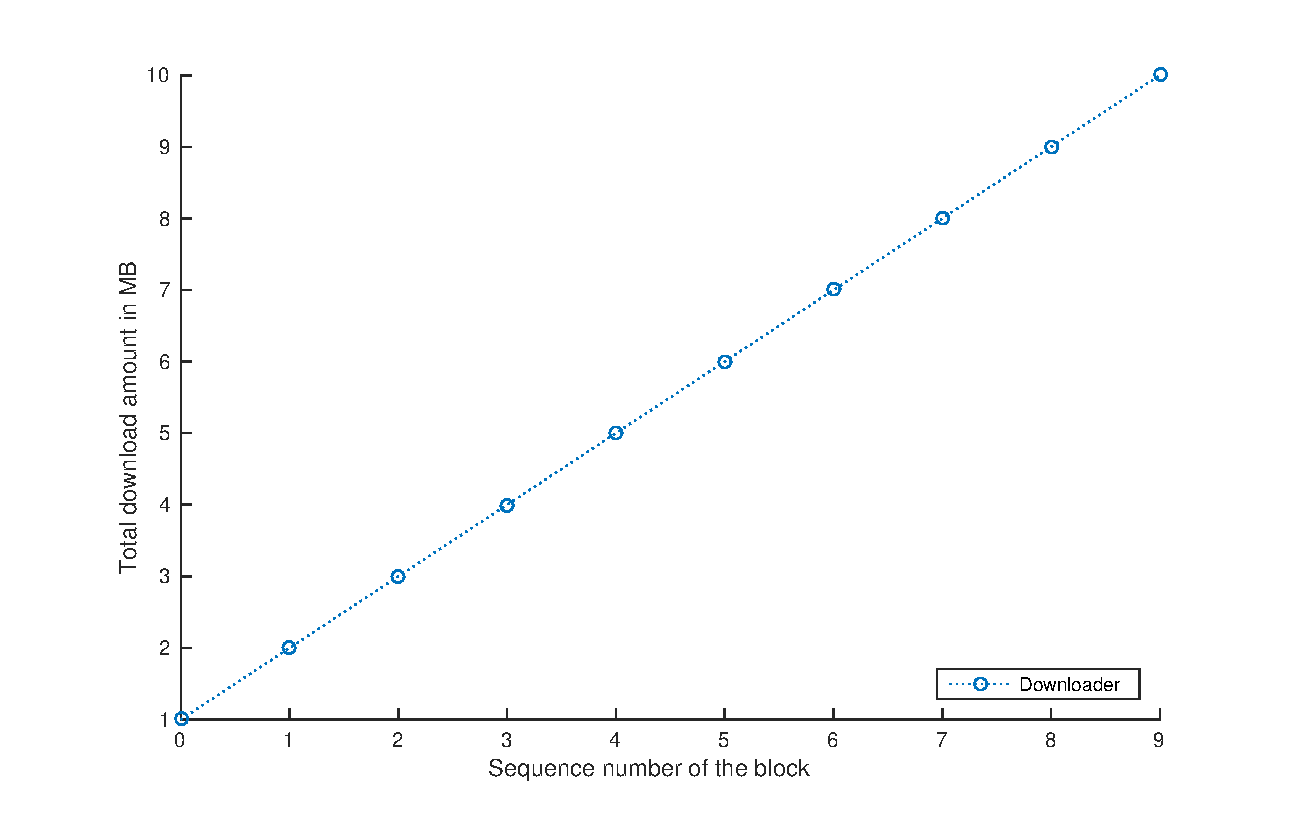
\includegraphics[scale=0.5]{experimentation/chain/small/chain-down.eps}}
\caption{Total download amount when creating a chain of 10 blocks for a 10MB download..}
\label{fig:chain-experiment-amounts-small}
\end{figure}

We also experimented with MutliChain running much longer with a bigger download.
Our next synthetic experiment we simulate a download of 10 GB with a speed of 1000 KB/s.
The rest of the setup is the same as in the previous example
and the result is plotted in the same way in Figure \ref{fig:chain-experiment-amounts-long}.
The individual points are obscured by the large amount of points in the figure.
The graph of the MultiChain would look identical to Figure \ref{fig:chain-experiment-graph},
except it would be 10000 blocks long.
It is not pictured as it is impractical to picture a chain of this length.
As can be seen in the plots, MultiChain has no problem running for a longer period of time.

\begin{figure}
\centerline{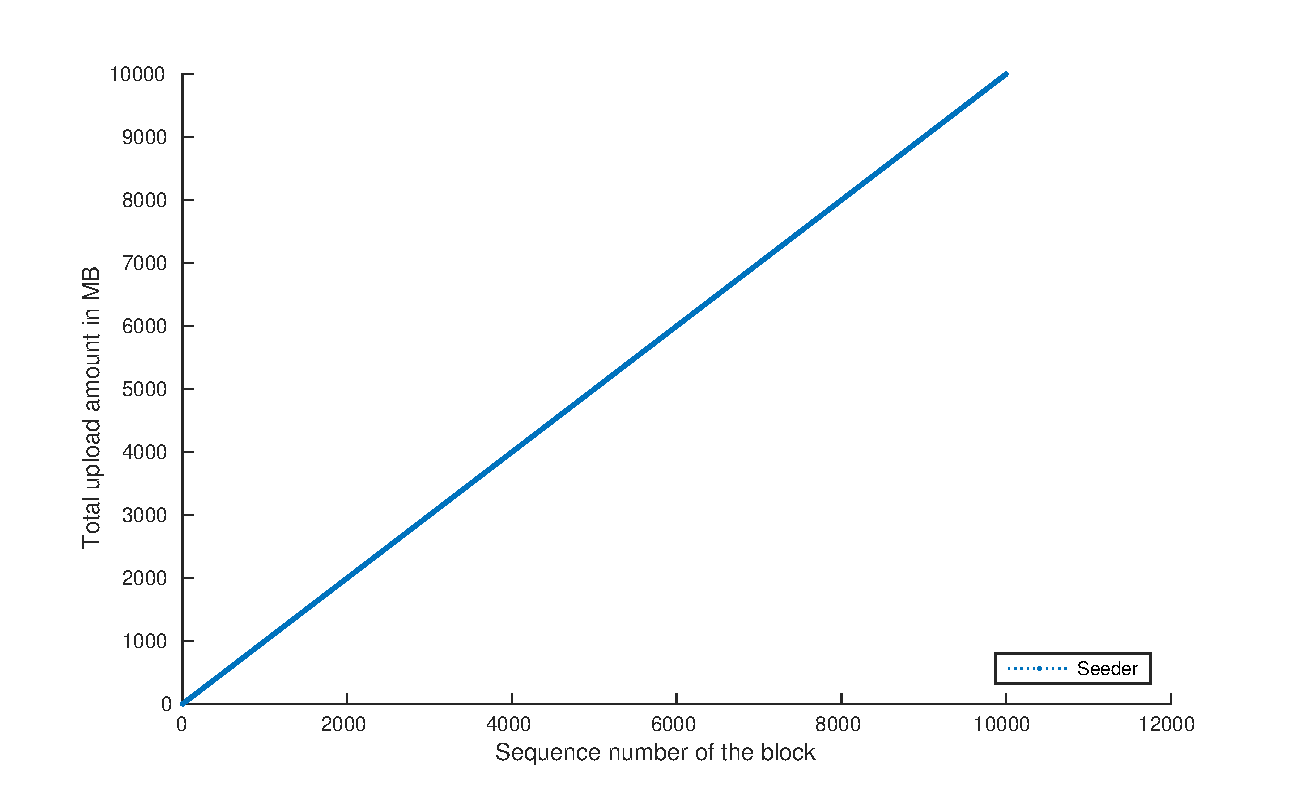
\includegraphics[scale=0.5]{experimentation/chain/long/chain-down.eps}}
\caption{Total download amount when creating a chain of 10 000 blocks for a 10GB download.}
\label{fig:chain-experiment-amounts-long}
\end{figure}